\section{Introduction}\label{sec:intro}
Cloud computing systems like Hadoop [ref], and Spark[ref] have been widely 
used in many companies such as Google, Yahoo, Facebook, and Microsoft. Their popularity 
brings forth new problems in the realm of task scheduling and management in these systems,
particularly with the rise of the cloud as a platform to host these frameworks.

In this paper, we explore the problem of sharing a cluster between users while preserving 
the efficiency of systems like Hadoop and Spark --- specifically, finding a trade-off 
between locality (i.e., the placement of computation near its input data) and fairness. 
Locality is important for task (and thus job) performance, as it reduces the amount of data 
that needs to travel across the network, while fairness is important for clusters to be 
useful to multiple users at load. 

Figure~\ref{fig:cluster}  demonstrates these tradeoffs between data locality and fairness,
in a simple four-machine cluster. We consider a
scenario where a "job" consists of many smaller tasks, and each node in the cluster 
has a finite number of "slots" which provide resources for tasks. Every task has input data,
located in some distributed file system in blocks across the cluster. When a slot
becomes available (a slot representing the resources to run a single task),
a scheduler that provides fair sharing needs to schedule tasks from the job 
that is farthest below its fair share first. In Figure 1, the job furthest below
the fair share is clearly Job 1, so a task from Job 1 will be chosen for the empty slot; however,
Job 1 has no input data on Machine 3, meaning that the task will need to transfer a block
of data over the network in order to proceed, incurring additional overhead and causing
worse performance. The question becomes: what should a fair scheduler do
in this situation? Should it sacrifice performance to enforce fairness, or choose another task
with local data and remedy the fairness imbalance later? 

\begin{figure}[t]
    \minipage{0.5\textwidth}
        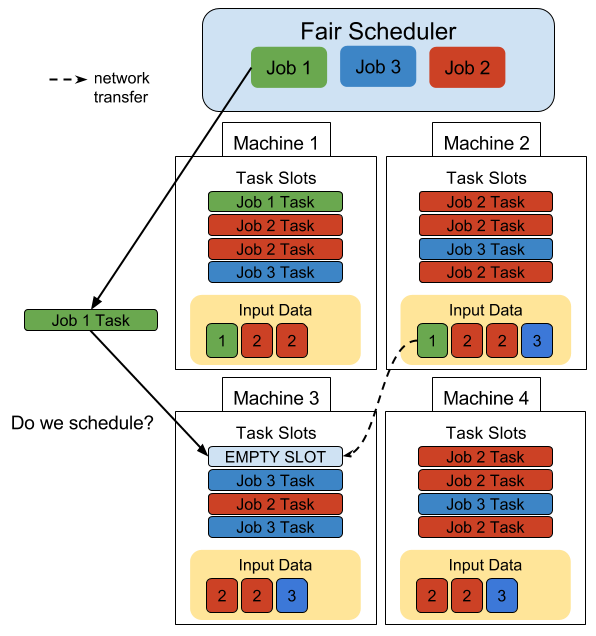
\includegraphics[width=\linewidth]{./fig1.png}
        \caption{A compute cluster, with a fair scheduler that must fill an empty slot}
        \label{fig:cluster}
    \endminipage
\end{figure}

The Hadoop Fair Scheduler (HFS) is an influential example of a cluster framework 
scheduler that seeks to find this balance. The HFS was designed with two main goals: 
\textit{Fair sharing}: dividing resources using max-min fair sharing [ref] to achieve 
statistical multiplexing, and 
\textit{Data locality}: placing computations (tasks) near their input data as often as
possible, to maximize system throughput.

To achieve the first goal (fair sharing), a scheduler must reallocate resources between 
jobs when the number of jobs changes; however, a strict implementation of fair sharing 
compromises locality, because the job to be scheduled next according to fairness might not
have data on the nodes that are currently free. To resolve this problem, the HFS relaxes 
fairness slightly through a simple algorithm called 
\textit{delay scheduling}~\cite{Zaharia:2010}, in which a 
job waits for a fixed amount of time for additional scheduling opportunities on nodes 
that have data for it, if none are available.

The original delay scheduling work [ref] reported that a small amount of waiting is enough
to bring locality close to 100\% (the chosen default value is three seconds). Since its 
inception, delay scheduling has been used in other cluster framekwork schedulers, such as 
Spark, as well as in resource managers, such as YARN[ref] and Mesos[ref]. 

Delay scheduling provides a simple solution for the scenario in 
Figure~\ref{fig:cluster}. Job 1 will simply be delayed for a fixed interval (and a task
from Job 3 scheduled in its place) in the hopes that data-local slots will open up in 
the future; however, delay scheduling assumes that data locality is always beneficial.
In reality, the decision is not as simple. The importance of data locality depends on many
factors, such as network conditions, input data size, disk i/o usage, and others. These
conditions may change over time (or even during the execution of a job). As well, with clusters
in the public cloud becoming so common, cluster conditions can change as simultaneous user
load changes, or after instances are stopped and restarted, potentially in a different physical
configuration. So, the
decision of whether or not to delay (and for how long) can not be efficiently solved with
a fixed, unchanging delay interval. We propose that an \emph{adaptive} mechanism is needed,
in order to properly judge and exploit these tradeoffs between fairness and locality,
based on feedback from the system.

In this paper, we present Dynamic Delay Scheduling, a simple, low-state, adaptive
solution for task scheduling in the cloud, which improves job latency over
fixed-interval delay scheduling. Dynamic Delay Scheduling operates by using feedback from finished
tasks in the system, which report their perceived overhead from remote data
reads. Our scheduler then adapts the delay scheduling interval to be used to schedule subsequent
tasks, using a running average of the overhead metrics reported as the interval
itself. In this way, our adaptive solution minimizes completion time by finding the shifting balance between:
1) immediate fairness policy enforcement, and 2) waiting for data locality, based on the severity of network overhead,
for increased performance.
This paper contributes an outline of this adaptive solution. We have
also implemented a simple prototype in Spark. Preliminary experiments demonstrate that
an adaptive delay outperforms the current Spark distribution (which uses a fixed delay
scheduling interval) in TPC-H workloads. 
%\textbf{Ideally, we need to identify some concrete statement concerning job latency and how it is minimized by DDS}

The remainder of this paper is structured in the following way. Section~\ref{sec:background}
presents background on fixed delay scheduling as a concept. Section~\ref{sec:systems} discusses how fixed delay
scheduling is implemented/mapped to real systems. Section~\ref{sec:dynamic} defines the terminology and
design of Dynamic Delay Scheduling, our simple adaptive scheduling solution. Section~\ref{sec:impl} describes our
lightweight implementation in Apache Spark. Section~\ref{sec:eval} demonstrates our evaluation of Dynamic
Delay Scheduling, using our implementation in Spark under several workloads. Finally, 
Section~\ref{sec:conclusion} provides closing remarks, and well as some future direction for further
applying adaptive algorithms to other facets of task scheduling.
%\textbf{Say a few words about expanding this work on adaptive algorithms}

